\documentclass{exam}
\usepackage[utf8]{inputenc}

\usepackage[dvipsnames]{xcolor}
\usepackage{microtype}
\usepackage{siunitx}
\DeclareSIUnit\year{yr}
\usepackage{pgfplots}
\usepackage{graphicx}
\usepackage{float}

\renewcommand*{\thefootnote}{\fnsymbol{footnote}}


\begin{document}

\section*{NCEA Level 1 Science (Genetics \#2)}

This worksheet is on inheritance and genetic variation.

\subsection*{Questions}
\begin{questions}
  \question What is the difference between a phenotype and a genotype?
  \question In pea plants, purple flowers (P) are dominant to white flowers (p). Give the genotype of
            a plant with white flowers. Is the genotype heterozygous or homozygous?
  \question A person with dimpled cheeks has the genotype DD or Dd. A person with smooth cheeks has the genotype dd. Which
            trait is dominant? If two people with dimpled cheeks carrying the recessive gene reproduce, what is the chance of
            the offspring having smooth cheeks?
  \question Explain why `pure breeders' always have a homozygous genotype.
  \question White colour is the dominant trait in sheep. Explain, with reference to a Punnett square, how a white ram and a
            white ewe could have a black lamb.
  \question Jim is able to taste the bitter chemical in the pith of a grapefruit (white layer between skin and fruit) but Emma
            cannot. They have four children; Jack and Anna can taste the fruit, but Mary and Peter cannot. The dominant trait
            is tasting (B).
    \begin{parts}
       \part Give the genome for each family member.
       \part Explain your genome choice for Jim, Emma, and Anna.
       \part Suppose Peter has a child with Sonya. What is the chance that their offspring is able to taste the chemical?
    \end{parts}
  \question {[NZQA 2017]} Piebaldism is a genetic condition causing a white patch on the head and body of horses. In horses 
            piebaldism is a dominant trait (H), and ``normal'' colour is recessive (h).
            
            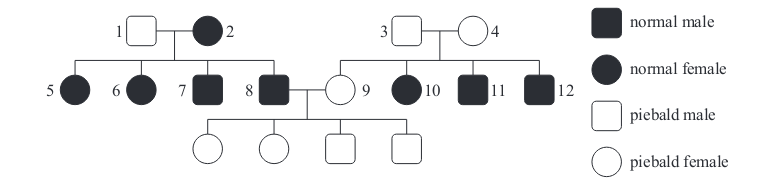
\includegraphics[width=\textwidth]{piebald}
            
    \begin{parts}
      \part From the pedigree chart above, list all the possible phenotypes and genotypes of horses 3, 8, and 9. 
      \part A breeder wants to produce only dominant (piebald) offspring from a breeding pair of horses. The breeder has piebald
            and normal horses to breed from. How could the breeder use crosses to make sure that the pair of horses were pure breeding?
    \end{parts}
\end{questions}

\clearpage
\subsection*{Homework}
\begin{questions}
  \question {[NZQA 2016]} The Venus flytrap plants come in a number of different types, such as the “B-52” with a red leaf. A teacher brought
            two identical plants to class and put them in different parts of the classroom. The Venus flytrap put near a window grew short leaves and
            the Venus flytrap in the shade grew long leaves. Colour variation in the leaves of the Venus flytraps can be passed on to a plant’s
            offspring, but the different leaf length cannot. Explain why.
            
            In your answer you should:
            \begin{itemize}
              \item define inheritable and non-inheritable variation
              \item explain what causes inheritable and non-inheritable variations.
            \end{itemize}
  \question {[NZQA 2016]} Photic sneezing is a condition which causes affected people to sneeze due to bright light. It can be traced
            through a family, as shown in the pedigree chart. Photic sneezing (A) is dominant to unaffected (a).
            
            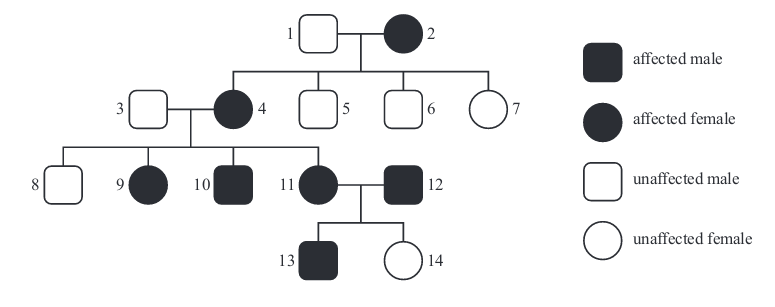
\includegraphics[width=\textwidth]{sneeze}
            
    \begin{parts}
      \part Work out the genomes of individuals 1, 2, 11, and 12.
      \part Explain how the pedigree chart can be used to show that Photic sneezing is dominant, but it cannot be used to determine the
            genotype of individual 13. You may use a Punnett square.
    \end{parts}
            
\end{questions}

\end{document}
